\documentclass[aspectratio=169,11pt]{beamer}
% =====================================================================
%  pds-beamer.tex — Estilo común de las transparencias.
%
%  Uso (desde teoría/Tx/transparencias/):
%     \documentclass[aspectratio=169,11pt]{beamer}
%     % =====================================================================
%  pds-beamer.tex — Estilo común de las transparencias.
%
%  Uso (desde teoría/Tx/transparencias/):
%     \documentclass[aspectratio=169,11pt]{beamer}
%     % =====================================================================
%  pds-beamer.tex — Estilo común de las transparencias.
%
%  Uso (desde teoría/Tx/transparencias/):
%     \documentclass[aspectratio=169,11pt]{beamer}
%     \input{../../comun/pds-beamer}
%     \title{...}  \subtitle{Tema x · ...}
%     \begin{document}
%       \portada
%       ...
%     \end{document}
%  Compilar con:  latexmk -xelatex  (o «make» desde teoría/)
% =====================================================================

\usetheme{Boadilla}
\usecolortheme{orchid}
\usefonttheme{professionalfonts}
\setbeamercovered{transparent}
\setbeamersize{text margin left=0.8cm, text margin right=0.8cm}
\setbeamertemplate{navigation symbols}{}
\setbeamertemplate{itemize item}[square]
\setbeamertemplate{itemize subitem}[circle]
\setbeamertemplate{itemize subsubitem}[triangle]
\setbeamertemplate{enumerate item}[square]
\setbeamertemplate{enumerate subitem}[circle]
\setbeamertemplate{caption}{\raggedright\insertcaption\par}

\input{../../comun/pds-comun.tex}

% Tipografía: Fira Sans + Fira Math (legibles en proyector)
\usepackage{fontspec}
\usepackage{unicode-math}
% Se cargan por nombre de fichero para que funcionen con cualquier
% instalación de TeX Live (o MiKTeX) sin instalar fuentes en el sistema.
\setmainfont{FiraSans}[Extension=.otf, UprightFont=*-Regular, BoldFont=*-SemiBold,
  ItalicFont=*-Italic, BoldItalicFont=*-SemiBoldItalic]
\setsansfont{FiraSans}[Extension=.otf, UprightFont=*-Regular, BoldFont=*-SemiBold,
  ItalicFont=*-Italic, BoldItalicFont=*-SemiBoldItalic]
\setmonofont{FiraMono}[Extension=.otf, UprightFont=*-Regular, BoldFont=*-Medium, AutoFakeSlant=0.15, Scale=0.92]
\setmathfont{FiraMath-Regular.otf}
\setmathfont{latinmodern-math.otf}[range={"229B,"22EE,"22F1}]

% Colores del tema ajustados a la paleta común (más contraste)
\setbeamercolor{structure}{fg=pdsazul}
\setbeamercolor{alerted text}{fg=pdsrojo}
\setbeamercolor{example text}{fg=pdsverde}
\setbeamercolor{block title}{bg=pdsazul, fg=white}
\setbeamercolor{block body}{bg=pdsfondo}
\setbeamercolor{block title alerted}{bg=pdsrojo, fg=white}
\setbeamercolor{block body alerted}{bg=pdsrojo!6}
\setbeamercolor{block title example}{bg=pdsverde, fg=white}
\setbeamercolor{block body example}{bg=pdsverde!6}
\setbeamercolor{frametitle}{fg=pdsazul, bg=white}
\setbeamerfont{frametitle}{size=\large, series=\bfseries}
\setbeamerfont{block title}{size=\normalsize, series=\bfseries}
\setbeamertemplate{blocks}[rounded][shadow=false]

% Logo en la esquina superior derecha de cada transparencia
\pgfdeclareimage[height=0.8cm]{logo}{../../comun/ucm.png}
\addtobeamertemplate{frametitle}{}{%
  \begin{tikzpicture}[remember picture, overlay]
    \node[anchor=north east, inner sep=0pt] at ([xshift=-0.25cm, yshift=-0.2cm]current page.north east) {\pgfuseimage{logo}};
  \end{tikzpicture}}

% Datos de portada
\author[\autorescorto]{\autores}
\institute[UCM]{\footnotesize\departamento\\\universidad}
\date[\curso]{\footnotesize\grado\\\curso}

\newcommand{\portada}{%
  \begin{frame}[plain]
    \begin{center}
      
\includegraphics[height=1.9cm]{../../comun/ucm.png}
    \end{center}
    \vspace{-0.4cm}
    \titlepage
  \end{frame}}

% Índice al empezar cada sección
\AtBeginSection[]{%
  \begin{frame}{Contenido}
    \tableofcontents[currentsection, hideothersubsections]
  \end{frame}}

\renewcommand{\pdscodesize}{\scriptsize}

% Utilidades
% \herramienta{T1-convolucion-continua}: enlace a la página publicada de
% herramientas/html (se abre en el navegador, sin instalar nada).
% \herramientaservidor{server/....py}: app que necesita Python (bokeh serve).
\newcommand{\urlherramientas}{https://ucm-237.github.io/PdS/}
\newcommand{\herramienta}[1]{%
  \par\vfill\hfill{\scriptsize\color{pdsgris}\faIcon\ \href{\urlherramientas#1.html}{Herramienta interactiva: \texttt{#1}}}}
\newcommand{\herramientaservidor}[1]{%
  \par\vfill\hfill{\scriptsize\color{pdsgris}\faIcon\ Herramienta interactiva (con Python): \texttt{herramientas/#1}}}
\newcommand{\faIcon}{\textbf{▶}}
\newcommand{\gris}[1]{{\color{pdsgris}#1}}
\newcommand{\nota}[1]{\par\vspace{2pt}{\footnotesize\color{pdsgris}\textit{#1}}\par}
% Nota sobre una errata de versiones anteriores (solo con \ERRATAS)
\newcommand{\errata}[1]{\iferratas\nota{Errata de versiones anteriores: #1}\fi}
\newcommand{\apuntes}[1]{\nota{Más detalle en los apuntes, #1.}}

% Bloques con nombre en castellano
\newenvironment{definicion}[1][Definición]{\begin{block}{#1}}{\end{block}}
\newenvironment{importante}[1][Importante]{\begin{alertblock}{#1}}{\end{alertblock}}
\newenvironment{ejemplo}[1][Ejemplo]{\begin{exampleblock}{#1}}{\end{exampleblock}}

%     \title{...}  \subtitle{Tema x · ...}
%     \begin{document}
%       \portada
%       ...
%     \end{document}
%  Compilar con:  latexmk -xelatex  (o «make» desde teoría/)
% =====================================================================

\usetheme{Boadilla}
\usecolortheme{orchid}
\usefonttheme{professionalfonts}
\setbeamercovered{transparent}
\setbeamersize{text margin left=0.8cm, text margin right=0.8cm}
\setbeamertemplate{navigation symbols}{}
\setbeamertemplate{itemize item}[square]
\setbeamertemplate{itemize subitem}[circle]
\setbeamertemplate{itemize subsubitem}[triangle]
\setbeamertemplate{enumerate item}[square]
\setbeamertemplate{enumerate subitem}[circle]
\setbeamertemplate{caption}{\raggedright\insertcaption\par}

% =====================================================================
%  pds-comun.tex — Paquetes, colores y estilos de código comunes a
%  transparencias, apuntes y hojas de ejercicios. Compilar con XeLaTeX.
%  No cargar directamente: lo cargan pds-beamer.tex y pds-apuntes.tex.
% =====================================================================

\usepackage{polyglossia}
\setmainlanguage{spanish}
\usepackage{mathtools}
\usepackage{graphicx}
\usepackage{booktabs}
\usepackage{multirow}
\usepackage{array}
\usepackage{xcolor}
\usepackage{tikz}
\usetikzlibrary{positioning,arrows.meta,calc,shapes.geometric,decorations.pathreplacing}
\usepackage{listings}
\usepackage{siunitx}
\sisetup{output-decimal-marker={,}, group-separator={\,}, per-mode=symbol}

% Notas de erratas de versiones anteriores: no se imprimen salvo que se
% defina \ERRATAS antes de cargar el estilo (make ERRATAS=1)
\newif\iferratas
\ifdefined\ERRATAS \erratastrue \fi

% Ruta común (logo y figuras compartidas)
\providecommand{\rutacomun}{../../comun/}
\input{\rutacomun datos.tex}

% ---------------------------------------------------------------------
%  Paleta (la misma que usan las figuras generadas con Python,
%  ver comun/pds_estilo.py)
% ---------------------------------------------------------------------
\definecolor{pdsazul}{HTML}{2B3A8C}
\definecolor{pdsrojo}{HTML}{C0392B}
\definecolor{pdsverde}{HTML}{1E7B4F}
\definecolor{pdsnaranja}{HTML}{D9822B}
\definecolor{pdsgris}{HTML}{5A5A66}
\definecolor{pdsfondo}{HTML}{F3F4FA}
\definecolor{pdscodigo}{HTML}{F7F7F2}

% ---------------------------------------------------------------------
%  Diagramas de bloques (TikZ)
% ---------------------------------------------------------------------
\tikzset{
  bloque/.style={rectangle, rounded corners=2pt, draw=pdsazul!80, fill=pdsfondo,
                 very thick, minimum height=8mm, minimum width=14mm, align=center},
  sumador/.style={circle, draw=pdsazul!80, fill=pdsfondo, thick, inner sep=1.5pt},
  flecha/.style={-{Stealth[length=2.2mm]}, thick, pdsgris},
}

% ---------------------------------------------------------------------
%  Código: Python y Matlab en paralelo
% ---------------------------------------------------------------------
\newcommand{\pdscodesize}{\footnotesize}
\lstdefinestyle{pds}{
  basicstyle=\ttfamily\pdscodesize,
  keywordstyle=\color{pdsazul}\bfseries,
  commentstyle=\color{pdsverde}\itshape,
  stringstyle=\color{pdsrojo},
  numbers=none,
  backgroundcolor=\color{pdscodigo},
  frame=single, rulecolor=\color{pdsgris!40}, framerule=0.4pt,
  xleftmargin=2pt, xrightmargin=2pt, aboveskip=2pt, belowskip=2pt,
  columns=fullflexible, keepspaces=true,
  showstringspaces=false, breaklines=true, tabsize=4,
  upquote=true,
  % Con XeLaTeX, listings desordena los caracteres no ASCII junto a
  % dígitos («2π» sale «π2»): se sustituyen por su versión matemática.
  literate={π}{{$\pi$}}1 {δ}{{$\delta$}}1 {ω}{{$\omega$}}1 {Ω}{{$\Omega$}}1
           {≈}{{$\approx$}}1 {µ}{{$\mu$}}1 {·}{{$\cdot$}}1 {α}{{$\alpha$}}1
           {á}{{á}}1 {é}{{é}}1 {í}{{í}}1 {ó}{{ó}}1 {ú}{{ú}}1 {ñ}{{ñ}}1 {¿}{{¿}}1,
}
\lstdefinestyle{python}{style=pds, language=Python,
  morekeywords={as,True,False,None}}
\lstdefinestyle{matlab}{style=pds, language=Matlab,
  morekeywords={function,end,true,false}}

% \codigo{<ruta sin extensión>} muestra el mismo ejemplo en Python
% y en Matlab, uno al lado del otro. Los ficheros viven en
% ../codigo/python/<nombre>.py y ../codigo/matlab/<nombre>.m y se
% ejecutan en las pruebas (make prueba-codigo).
\newcommand{\rutacodigo}{../codigo/}
\newcommand{\codigoetiqueta}[1]{{\sffamily\scriptsize\bfseries\color{pdsgris}#1}}
\newcommand{\codigo}[2][]{%
  \par\noindent
  \begin{minipage}[t]{0.495\linewidth}
    \codigoetiqueta{Python}\par\vspace{1pt}
    \lstinputlisting[style=python,#1]{\rutacodigo python/#2.py}
  \end{minipage}\hfill
  \begin{minipage}[t]{0.495\linewidth}
    \codigoetiqueta{Matlab}\par\vspace{1pt}
    \lstinputlisting[style=matlab,#1]{\rutacodigo matlab/#2.m}
  \end{minipage}\par}

\input{\rutacomun notacion.tex}


% Tipografía: Fira Sans + Fira Math (legibles en proyector)
\usepackage{fontspec}
\usepackage{unicode-math}
% Se cargan por nombre de fichero para que funcionen con cualquier
% instalación de TeX Live (o MiKTeX) sin instalar fuentes en el sistema.
\setmainfont{FiraSans}[Extension=.otf, UprightFont=*-Regular, BoldFont=*-SemiBold,
  ItalicFont=*-Italic, BoldItalicFont=*-SemiBoldItalic]
\setsansfont{FiraSans}[Extension=.otf, UprightFont=*-Regular, BoldFont=*-SemiBold,
  ItalicFont=*-Italic, BoldItalicFont=*-SemiBoldItalic]
\setmonofont{FiraMono}[Extension=.otf, UprightFont=*-Regular, BoldFont=*-Medium, AutoFakeSlant=0.15, Scale=0.92]
\setmathfont{FiraMath-Regular.otf}
\setmathfont{latinmodern-math.otf}[range={"229B,"22EE,"22F1}]

% Colores del tema ajustados a la paleta común (más contraste)
\setbeamercolor{structure}{fg=pdsazul}
\setbeamercolor{alerted text}{fg=pdsrojo}
\setbeamercolor{example text}{fg=pdsverde}
\setbeamercolor{block title}{bg=pdsazul, fg=white}
\setbeamercolor{block body}{bg=pdsfondo}
\setbeamercolor{block title alerted}{bg=pdsrojo, fg=white}
\setbeamercolor{block body alerted}{bg=pdsrojo!6}
\setbeamercolor{block title example}{bg=pdsverde, fg=white}
\setbeamercolor{block body example}{bg=pdsverde!6}
\setbeamercolor{frametitle}{fg=pdsazul, bg=white}
\setbeamerfont{frametitle}{size=\large, series=\bfseries}
\setbeamerfont{block title}{size=\normalsize, series=\bfseries}
\setbeamertemplate{blocks}[rounded][shadow=false]

% Logo en la esquina superior derecha de cada transparencia
\pgfdeclareimage[height=0.8cm]{logo}{../../comun/ucm.png}
\addtobeamertemplate{frametitle}{}{%
  \begin{tikzpicture}[remember picture, overlay]
    \node[anchor=north east, inner sep=0pt] at ([xshift=-0.25cm, yshift=-0.2cm]current page.north east) {\pgfuseimage{logo}};
  \end{tikzpicture}}

% Datos de portada
\author[\autorescorto]{\autores}
\institute[UCM]{\footnotesize\departamento\\\universidad}
\date[\curso]{\footnotesize\grado\\\curso}

\newcommand{\portada}{%
  \begin{frame}[plain]
    \begin{center}
      
\includegraphics[height=1.9cm]{../../comun/ucm.png}
    \end{center}
    \vspace{-0.4cm}
    \titlepage
  \end{frame}}

% Índice al empezar cada sección
\AtBeginSection[]{%
  \begin{frame}{Contenido}
    \tableofcontents[currentsection, hideothersubsections]
  \end{frame}}

\renewcommand{\pdscodesize}{\scriptsize}

% Utilidades
% \herramienta{T1-convolucion-continua}: enlace a la página publicada de
% herramientas/html (se abre en el navegador, sin instalar nada).
% \herramientaservidor{server/....py}: app que necesita Python (bokeh serve).
\newcommand{\urlherramientas}{https://ucm-237.github.io/PdS/}
\newcommand{\herramienta}[1]{%
  \par\vfill\hfill{\scriptsize\color{pdsgris}\faIcon\ \href{\urlherramientas#1.html}{Herramienta interactiva: \texttt{#1}}}}
\newcommand{\herramientaservidor}[1]{%
  \par\vfill\hfill{\scriptsize\color{pdsgris}\faIcon\ Herramienta interactiva (con Python): \texttt{herramientas/#1}}}
\newcommand{\faIcon}{\textbf{▶}}
\newcommand{\gris}[1]{{\color{pdsgris}#1}}
\newcommand{\nota}[1]{\par\vspace{2pt}{\footnotesize\color{pdsgris}\textit{#1}}\par}
% Nota sobre una errata de versiones anteriores (solo con \ERRATAS)
\newcommand{\errata}[1]{\iferratas\nota{Errata de versiones anteriores: #1}\fi}
\newcommand{\apuntes}[1]{\nota{Más detalle en los apuntes, #1.}}

% Bloques con nombre en castellano
\newenvironment{definicion}[1][Definición]{\begin{block}{#1}}{\end{block}}
\newenvironment{importante}[1][Importante]{\begin{alertblock}{#1}}{\end{alertblock}}
\newenvironment{ejemplo}[1][Ejemplo]{\begin{exampleblock}{#1}}{\end{exampleblock}}

%     \title{...}  \subtitle{Tema x · ...}
%     \begin{document}
%       \portada
%       ...
%     \end{document}
%  Compilar con:  latexmk -xelatex  (o «make» desde teoría/)
% =====================================================================

\usetheme{Boadilla}
\usecolortheme{orchid}
\usefonttheme{professionalfonts}
\setbeamercovered{transparent}
\setbeamersize{text margin left=0.8cm, text margin right=0.8cm}
\setbeamertemplate{navigation symbols}{}
\setbeamertemplate{itemize item}[square]
\setbeamertemplate{itemize subitem}[circle]
\setbeamertemplate{itemize subsubitem}[triangle]
\setbeamertemplate{enumerate item}[square]
\setbeamertemplate{enumerate subitem}[circle]
\setbeamertemplate{caption}{\raggedright\insertcaption\par}

% =====================================================================
%  pds-comun.tex — Paquetes, colores y estilos de código comunes a
%  transparencias, apuntes y hojas de ejercicios. Compilar con XeLaTeX.
%  No cargar directamente: lo cargan pds-beamer.tex y pds-apuntes.tex.
% =====================================================================

\usepackage{polyglossia}
\setmainlanguage{spanish}
\usepackage{mathtools}
\usepackage{graphicx}
\usepackage{booktabs}
\usepackage{multirow}
\usepackage{array}
\usepackage{xcolor}
\usepackage{tikz}
\usetikzlibrary{positioning,arrows.meta,calc,shapes.geometric,decorations.pathreplacing}
\usepackage{listings}
\usepackage{siunitx}
\sisetup{output-decimal-marker={,}, group-separator={\,}, per-mode=symbol}

% Notas de erratas de versiones anteriores: no se imprimen salvo que se
% defina \ERRATAS antes de cargar el estilo (make ERRATAS=1)
\newif\iferratas
\ifdefined\ERRATAS \erratastrue \fi

% Ruta común (logo y figuras compartidas)
\providecommand{\rutacomun}{../../comun/}
\input{\rutacomun datos.tex}

% ---------------------------------------------------------------------
%  Paleta (la misma que usan las figuras generadas con Python,
%  ver comun/pds_estilo.py)
% ---------------------------------------------------------------------
\definecolor{pdsazul}{HTML}{2B3A8C}
\definecolor{pdsrojo}{HTML}{C0392B}
\definecolor{pdsverde}{HTML}{1E7B4F}
\definecolor{pdsnaranja}{HTML}{D9822B}
\definecolor{pdsgris}{HTML}{5A5A66}
\definecolor{pdsfondo}{HTML}{F3F4FA}
\definecolor{pdscodigo}{HTML}{F7F7F2}

% ---------------------------------------------------------------------
%  Diagramas de bloques (TikZ)
% ---------------------------------------------------------------------
\tikzset{
  bloque/.style={rectangle, rounded corners=2pt, draw=pdsazul!80, fill=pdsfondo,
                 very thick, minimum height=8mm, minimum width=14mm, align=center},
  sumador/.style={circle, draw=pdsazul!80, fill=pdsfondo, thick, inner sep=1.5pt},
  flecha/.style={-{Stealth[length=2.2mm]}, thick, pdsgris},
}

% ---------------------------------------------------------------------
%  Código: Python y Matlab en paralelo
% ---------------------------------------------------------------------
\newcommand{\pdscodesize}{\footnotesize}
\lstdefinestyle{pds}{
  basicstyle=\ttfamily\pdscodesize,
  keywordstyle=\color{pdsazul}\bfseries,
  commentstyle=\color{pdsverde}\itshape,
  stringstyle=\color{pdsrojo},
  numbers=none,
  backgroundcolor=\color{pdscodigo},
  frame=single, rulecolor=\color{pdsgris!40}, framerule=0.4pt,
  xleftmargin=2pt, xrightmargin=2pt, aboveskip=2pt, belowskip=2pt,
  columns=fullflexible, keepspaces=true,
  showstringspaces=false, breaklines=true, tabsize=4,
  upquote=true,
  % Con XeLaTeX, listings desordena los caracteres no ASCII junto a
  % dígitos («2π» sale «π2»): se sustituyen por su versión matemática.
  literate={π}{{$\pi$}}1 {δ}{{$\delta$}}1 {ω}{{$\omega$}}1 {Ω}{{$\Omega$}}1
           {≈}{{$\approx$}}1 {µ}{{$\mu$}}1 {·}{{$\cdot$}}1 {α}{{$\alpha$}}1
           {á}{{á}}1 {é}{{é}}1 {í}{{í}}1 {ó}{{ó}}1 {ú}{{ú}}1 {ñ}{{ñ}}1 {¿}{{¿}}1,
}
\lstdefinestyle{python}{style=pds, language=Python,
  morekeywords={as,True,False,None}}
\lstdefinestyle{matlab}{style=pds, language=Matlab,
  morekeywords={function,end,true,false}}

% \codigo{<ruta sin extensión>} muestra el mismo ejemplo en Python
% y en Matlab, uno al lado del otro. Los ficheros viven en
% ../codigo/python/<nombre>.py y ../codigo/matlab/<nombre>.m y se
% ejecutan en las pruebas (make prueba-codigo).
\newcommand{\rutacodigo}{../codigo/}
\newcommand{\codigoetiqueta}[1]{{\sffamily\scriptsize\bfseries\color{pdsgris}#1}}
\newcommand{\codigo}[2][]{%
  \par\noindent
  \begin{minipage}[t]{0.495\linewidth}
    \codigoetiqueta{Python}\par\vspace{1pt}
    \lstinputlisting[style=python,#1]{\rutacodigo python/#2.py}
  \end{minipage}\hfill
  \begin{minipage}[t]{0.495\linewidth}
    \codigoetiqueta{Matlab}\par\vspace{1pt}
    \lstinputlisting[style=matlab,#1]{\rutacodigo matlab/#2.m}
  \end{minipage}\par}

\input{\rutacomun notacion.tex}


% Tipografía: Fira Sans + Fira Math (legibles en proyector)
\usepackage{fontspec}
\usepackage{unicode-math}
% Se cargan por nombre de fichero para que funcionen con cualquier
% instalación de TeX Live (o MiKTeX) sin instalar fuentes en el sistema.
\setmainfont{FiraSans}[Extension=.otf, UprightFont=*-Regular, BoldFont=*-SemiBold,
  ItalicFont=*-Italic, BoldItalicFont=*-SemiBoldItalic]
\setsansfont{FiraSans}[Extension=.otf, UprightFont=*-Regular, BoldFont=*-SemiBold,
  ItalicFont=*-Italic, BoldItalicFont=*-SemiBoldItalic]
\setmonofont{FiraMono}[Extension=.otf, UprightFont=*-Regular, BoldFont=*-Medium, AutoFakeSlant=0.15, Scale=0.92]
\setmathfont{FiraMath-Regular.otf}
\setmathfont{latinmodern-math.otf}[range={"229B,"22EE,"22F1}]

% Colores del tema ajustados a la paleta común (más contraste)
\setbeamercolor{structure}{fg=pdsazul}
\setbeamercolor{alerted text}{fg=pdsrojo}
\setbeamercolor{example text}{fg=pdsverde}
\setbeamercolor{block title}{bg=pdsazul, fg=white}
\setbeamercolor{block body}{bg=pdsfondo}
\setbeamercolor{block title alerted}{bg=pdsrojo, fg=white}
\setbeamercolor{block body alerted}{bg=pdsrojo!6}
\setbeamercolor{block title example}{bg=pdsverde, fg=white}
\setbeamercolor{block body example}{bg=pdsverde!6}
\setbeamercolor{frametitle}{fg=pdsazul, bg=white}
\setbeamerfont{frametitle}{size=\large, series=\bfseries}
\setbeamerfont{block title}{size=\normalsize, series=\bfseries}
\setbeamertemplate{blocks}[rounded][shadow=false]

% Logo en la esquina superior derecha de cada transparencia
\pgfdeclareimage[height=0.8cm]{logo}{../../comun/ucm.png}
\addtobeamertemplate{frametitle}{}{%
  \begin{tikzpicture}[remember picture, overlay]
    \node[anchor=north east, inner sep=0pt] at ([xshift=-0.25cm, yshift=-0.2cm]current page.north east) {\pgfuseimage{logo}};
  \end{tikzpicture}}

% Datos de portada
\author[\autorescorto]{\autores}
\institute[UCM]{\footnotesize\departamento\\\universidad}
\date[\curso]{\footnotesize\grado\\\curso}

\newcommand{\portada}{%
  \begin{frame}[plain]
    \begin{center}
      
\includegraphics[height=1.9cm]{../../comun/ucm.png}
    \end{center}
    \vspace{-0.4cm}
    \titlepage
  \end{frame}}

% Índice al empezar cada sección
\AtBeginSection[]{%
  \begin{frame}{Contenido}
    \tableofcontents[currentsection, hideothersubsections]
  \end{frame}}

\renewcommand{\pdscodesize}{\scriptsize}

% Utilidades
% \herramienta{T1-convolucion-continua}: enlace a la página publicada de
% herramientas/html (se abre en el navegador, sin instalar nada).
% \herramientaservidor{server/....py}: app que necesita Python (bokeh serve).
\newcommand{\urlherramientas}{https://ucm-237.github.io/PdS/}
\newcommand{\herramienta}[1]{%
  \par\vfill\hfill{\scriptsize\color{pdsgris}\faIcon\ \href{\urlherramientas#1.html}{Herramienta interactiva: \texttt{#1}}}}
\newcommand{\herramientaservidor}[1]{%
  \par\vfill\hfill{\scriptsize\color{pdsgris}\faIcon\ Herramienta interactiva (con Python): \texttt{herramientas/#1}}}
\newcommand{\faIcon}{\textbf{▶}}
\newcommand{\gris}[1]{{\color{pdsgris}#1}}
\newcommand{\nota}[1]{\par\vspace{2pt}{\footnotesize\color{pdsgris}\textit{#1}}\par}
% Nota sobre una errata de versiones anteriores (solo con \ERRATAS)
\newcommand{\errata}[1]{\iferratas\nota{Errata de versiones anteriores: #1}\fi}
\newcommand{\apuntes}[1]{\nota{Más detalle en los apuntes, #1.}}

% Bloques con nombre en castellano
\newenvironment{definicion}[1][Definición]{\begin{block}{#1}}{\end{block}}
\newenvironment{importante}[1][Importante]{\begin{alertblock}{#1}}{\end{alertblock}}
\newenvironment{ejemplo}[1][Ejemplo]{\begin{exampleblock}{#1}}{\end{exampleblock}}

\graphicspath{{../figuras/}}

\title[T6 · Varias variables]{Señales aleatorias}
\subtitle{Tema 6 · Parte 2: varias variables aleatorias}

\begin{document}
\portada

% =====================================================================
\section{Distribución conjunta}

\begin{frame}{Varias variables a la vez}
  \small
  \begin{itemize}
    \item Muchas magnitudes aleatorias aparecen juntas: los valores de una señal en dos instantes, la entrada y la salida de un sistema, las coordenadas de un punto.
    \item Se describen con la \alert{distribución conjunta}:
    \[
      F_{XY}(x,y)=P(X\le x,\,Y\le y),\qquad f_{XY}(x,y)=\frac{\partial^2F_{XY}}{\partial x\,\partial y},
    \]
    \[
      P\big((X,Y)\in A\big)=\iint_Af_{XY}(x,y)\dd x\dd y .
    \]
    En discreto, $p_{XY}(x_i,y_j)=P(X=x_i,\,Y=y_j)$.
    \item Para $M$ variables, $f_{X_1\cdots X_M}(x_1,\dots,x_M)$, o con notación vectorial $f_{\mathbf X}(\mathbf x)$.
  \end{itemize}
\end{frame}

\begin{frame}{Marginales y condicionadas}
  \small
  \begin{itemize}
    \item \alert{Marginalización}: la distribución de una variable se obtiene integrando (o sumando) las demás:
    \[
      f_X(x)=\int_{-\infty}^{\infty}f_{XY}(x,y)\dd y,\qquad p_X(x_i)=\sum_jp_{XY}(x_i,y_j).
    \]
    \item \alert{Condicionada}: la distribución de $Y$ sabiendo que $X=x$,
    \[
      f_{Y|X}(y|x)=\frac{f_{XY}(x,y)}{f_X(x)} .
    \]
    \item \alert{Regla de la cadena}: $f_{XY}=f_{Y|X}\,f_X=f_{X|Y}\,f_Y$. Con $M$ variables hay $M!$ órdenes posibles:
    \(
      f(x_1,\dots,x_M)=f(x_1)\,f(x_2|x_1)\cdots f(x_M|x_1,\dots,x_{M-1}).
    \)
    \item \alert{Teorema de Bayes}: $f_{X|Y}(x|y)=\dfrac{f_{Y|X}(y|x)\,f_X(x)}{f_Y(y)}$.
  \end{itemize}
\end{frame}

\begin{frame}{Ejemplo: una conjunta construida por partes}
  \begin{center}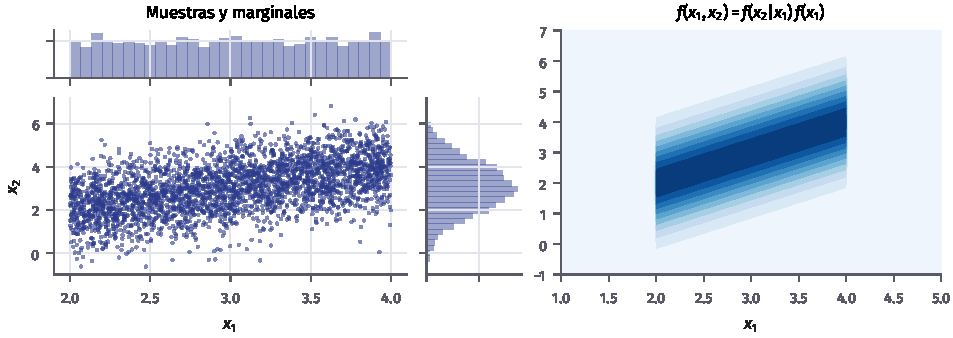
\includegraphics[width=0.9\linewidth]{conjunta}\end{center}
  \small
  $X_1\sim\mathcal U[2,4]$ y, dado $X_1=x_1$, $X_2\sim\mathcal N(x_1,1)$. Por la regla de la cadena,
  \(
    f(x_1,x_2)=\frac12\cdot\frac1{\sqrt{2\pi}}\e^{-(x_2-x_1)^2/2}
  \)
  en $2\le x_1\le4$. Para muestrear se sigue el mismo orden: primero $x_1$, después $x_2$ con ese $x_1$.
\end{frame}

\begin{frame}{Independencia}
  \begin{definicion}[Variables independientes]
    $X$ e $Y$ son independientes si $f_{XY}(x,y)=f_X(x)\,f_Y(y)$ para todo $(x,y)$, es decir, si $f_{Y|X}(y|x)=f_Y(y)$: saber $X$ no dice nada de $Y$.
  \end{definicion}
  \small
  \begin{itemize}
    \item $M$ variables son independientes si la conjunta es el producto de las $M$ marginales. Entonces basta muestrear cada una por separado.
    \item \alert{Independencia condicional}: $X$ e $Y$ son independientes dado $Z$ si $f_{XY|Z}=f_{X|Z}\,f_{Y|Z}$. Es la base de los modelos de Markov (parte~3).
    \item En el ejemplo anterior $X_1$ y $X_2$ \emph{no} son independientes: la media de $X_2$ depende de $X_1$.
  \end{itemize}
\end{frame}

% =====================================================================
\section{Correlación y covarianza}

\begin{frame}{Estadísticos de un par de variables}
  \small
  \begin{itemize}
    \item \alert{Correlación}: $R_{XY}=E\{XY\}=\iint xy\,f_{XY}(x,y)\dd x\dd y$.
    \item \alert{Covarianza}: $C_{XY}=E\{(X-\mu_X)(Y-\mu_Y)\}=R_{XY}-\mu_X\mu_Y$. $C_{XX}=\sigma_X^2$.
    \item \alert{Coeficiente de correlación}:
    \[
      \rho_{XY}=\frac{C_{XY}}{\sigma_X\sigma_Y},\qquad-1\le\rho_{XY}\le1 .
    \]
    Mide la dependencia \emph{lineal}: $\abs{\rho}=1$ si y solo si $Y=aX+b$; el signo es el de $a$.
    \item $X$ e $Y$ son \alert{incorreladas} si $C_{XY}=0$ (es decir, $E\{XY\}=\mu_X\mu_Y$), y \alert{ortogonales} si $R_{XY}=0$.
    \item Varianza de una suma: $\operatorname{Var}\{X+Y\}=\sigma_X^2+\sigma_Y^2+2C_{XY}$.
  \end{itemize}
  \nota{Las transparencias antiguas usaban $\phi$ para la correlación y $\psi$ para la covarianza; aquí $R$ y $C$, porque $\phi$ queda para las señales y $\psi$ para las wavelets (tema~5).}
\end{frame}

\begin{frame}{Incorreladas no es lo mismo que independientes}
  \begin{center}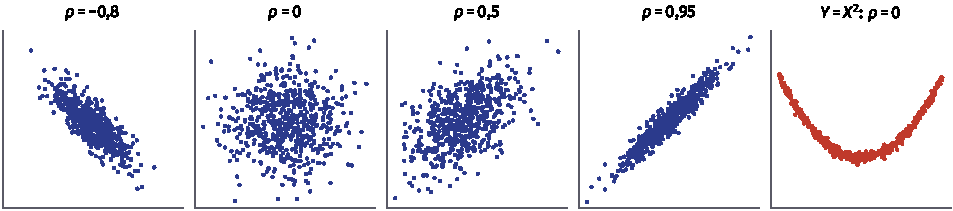
\includegraphics[width=\linewidth]{correlacion}\end{center}
  \small
  \begin{itemize}
    \item Independientes $\Rightarrow$ incorreladas: $E\{XY\}=\iint xy\,f_X f_Y=\mu_X\mu_Y$.
    \item Al revés no: con $X\sim\mathcal U[-1,1]$ e $Y=X^2$, $C_{XY}=E\{X^3\}-0=0$, aunque $Y$ es función de $X$.
    \item Por tanto: \alert{correladas $\Rightarrow$ dependientes}, pero la correlación nula no prueba la independencia. Excepción: variables \alert{conjuntamente gaussianas}.
  \end{itemize}
\end{frame}

\begin{frame}{En código: estimar media, covarianza y $\rho$}
  \codigo{conjunta}
  \nota{Teórico: $\mu_2=3$, $\sigma_2^2=1+\frac13$, $C_{12}=\operatorname{Var}\{X_1\}=\frac13$, $\rho=0{,}5$. \texttt{cov} divide por $N-1$; \texttt{corr} de Matlab necesita la Statistics Toolbox, \texttt{corrcoef} no.}
\end{frame}

% =====================================================================
\section{Vectores aleatorios y gaussiana multivariable}

\begin{frame}{Vector de medias y matriz de covarianza}
  \small
  Con $\mathbf X=(X_1,\dots,X_M)^T$:
  \[
    \boldsymbol\mu=E\{\mathbf X\},\qquad
    \boldsymbol\Sigma=E\{(\mathbf X-\boldsymbol\mu)(\mathbf X-\boldsymbol\mu)^T\}=
    \begin{bmatrix}\sigma_1^2&C_{12}&\cdots&C_{1M}\\C_{12}&\sigma_2^2&\cdots&C_{2M}\\\vdots&&\ddots&\vdots\\C_{1M}&C_{2M}&\cdots&\sigma_M^2\end{bmatrix}
  \]
  \begin{itemize}
    \item $\boldsymbol\Sigma$ es simétrica y semidefinida positiva; diagonal si las variables están incorreladas.
    \item \alert{Transformación lineal}: si $\mathbf Y=\mathbf A\mathbf X+\mathbf b$, entonces $\boldsymbol\mu_Y=\mathbf A\boldsymbol\mu+\mathbf b$ y $\boldsymbol\Sigma_Y=\mathbf A\boldsymbol\Sigma\mathbf A^T$.
    \item Estimación con $N$ muestras en las filas de una matriz $N\times M$: \texttt{mean(X)}, \texttt{cov(X)}, \texttt{corrcoef(X)}. En numpy, \texttt{np.cov} espera las variables en las filas.
  \end{itemize}
\end{frame}

\begin{frame}{Gaussiana multivariable}
  \begin{columns}[c]
    \begin{column}{0.5\textwidth}
      \small
      \[
        f_{\mathbf X}(\mathbf x)=\frac{\e^{-\frac12(\mathbf x-\boldsymbol\mu)^T\boldsymbol\Sigma^{-1}(\mathbf x-\boldsymbol\mu)}}{\sqrt{(2\pi)^M\det\boldsymbol\Sigma}}
      \]
      \begin{itemize}
        \item Queda determinada por $\boldsymbol\mu$ y $\boldsymbol\Sigma$.
        \item Curvas de nivel: elipses con ejes en los autovectores de $\boldsymbol\Sigma=\mathbf V\boldsymbol\Lambda\mathbf V^T$ y semiejes $\propto\sqrt{\lambda_k}$.
        \item Marginales, condicionadas y transformaciones lineales son gaussianas.
        \item Incorreladas $\Leftrightarrow$ $\boldsymbol\Sigma$ diagonal $\Leftrightarrow$ independientes.
      \end{itemize}
    \end{column}
    \begin{column}{0.48\textwidth}
      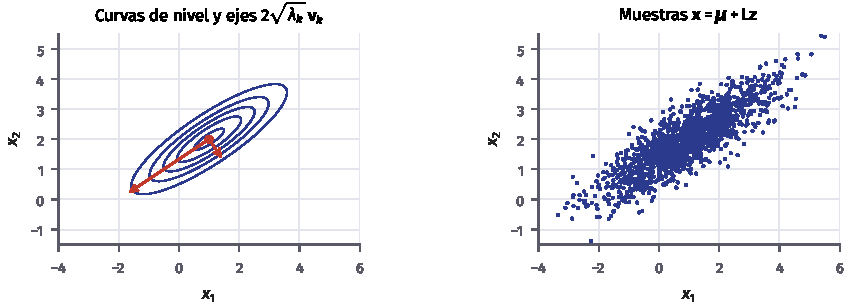
\includegraphics[width=\linewidth]{gaussiana2d}
      \nota{$\boldsymbol\mu=(1,2)$, $\boldsymbol\Sigma=\begin{bsmallmatrix}2&1{,}2\\1{,}2&1\end{bsmallmatrix}$: $\lambda=0{,}2$ y $2{,}8$, $\rho=0{,}85$.}
    \end{column}
  \end{columns}
\end{frame}

\begin{frame}{Muestrear una gaussiana multivariable}
  \small
  \begin{itemize}
    \item Se generan $M$ gaussianas $\mathcal N(0,1)$ independientes, $\mathbf z$, y se transforman: $\mathbf x=\boldsymbol\mu+\mathbf L\mathbf z$, con $\mathbf L\mathbf L^T=\boldsymbol\Sigma$. Por la transformación lineal, $\boldsymbol\Sigma_X=\mathbf L\mathbf I\mathbf L^T=\boldsymbol\Sigma$.
    \item $\mathbf L$: la factorización de Cholesky (\texttt{chol}) o $\mathbf V\boldsymbol\Lambda^{1/2}$ (\texttt{eig}): rotar y escalar.
  \end{itemize}
  \codigo[basicstyle=\ttfamily\fontsize{6.6}{7.5}\selectfont]{gaussiana_nd}
\end{frame}

% =====================================================================
\section{Suma de variables y teorema del límite central}

\begin{frame}{Suma de variables independientes}
  \begin{center}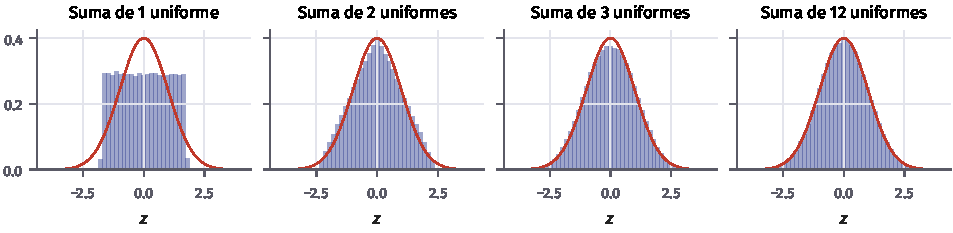
\includegraphics[width=0.8\linewidth]{tcl}\end{center}
  \small
  \begin{columns}[T]
    \begin{column}{0.5\textwidth}
      $S=X+Y$ con $X$ e $Y$ independientes:
      \begin{itemize}
        \item $\mu_S=\mu_X+\mu_Y$ (siempre); $\sigma_S^2=\sigma_X^2+\sigma_Y^2$ (basta incorreladas).
        \item $f_S=f_X\conv f_Y$: la densidad de la suma es la \alert{convolución} de las densidades. Dos $\mathcal U[0,1]$ dan un triángulo en $[0,2]$.
      \end{itemize}
    \end{column}
    \begin{column}{0.48\textwidth}
      \begin{importante}[Teorema del límite central]
        La suma de muchas variables independientes con varianza finita, normalizada, tiende a una gaussiana, sea cual sea su distribución.
      \end{importante}
      \nota{En la figura, $Z=(S-n/2)/\sqrt{n/12}$. Por eso el ruido térmico es gaussiano.}
    \end{column}
  \end{columns}
\end{frame}

% =====================================================================
\section*{Resumen}
\begin{frame}{Conceptos importantes}
  \begin{columns}[T]
    \begin{column}{0.5\textwidth}
      \begin{itemize}
        \item Conjunta, marginal (integrar), condicionada; cadena y Bayes.
        \item Independencia: la conjunta es el producto.
        \item $R_{XY}$, $C_{XY}=R_{XY}-\mu_X\mu_Y$, $\rho\in[-1,1]$.
        \item Independientes $\Rightarrow$ incorreladas; no al revés, salvo gaussianas.
      \end{itemize}
    \end{column}
    \begin{column}{0.5\textwidth}
      \begin{itemize}
        \item $\boldsymbol\mu$, $\boldsymbol\Sigma$; $\boldsymbol\Sigma_Y=\mathbf A\boldsymbol\Sigma\mathbf A^T$.
        \item Gaussiana multivariable; muestreo $\boldsymbol\mu+\mathbf L\mathbf z$.
        \item Suma: medias y varianzas se suman; densidades se convolucionan; TCL.
      \end{itemize}
    \end{column}
  \end{columns}
  \bigskip
  \gris{Apuntes del Tema 6, sección 2 · Hoja de ejercicios, ejercicios 6–10.}
\end{frame}

\end{document}
